%====================================================================%
%                  MORIOND.TEX                                       %
%====================================================================%



\documentclass{moriond}

\usepackage{lineno}
\linenumbers
\bibliographystyle{unsrt}    
% for BibTeX - sorted numerical labels by order of
% first citation.

% A useful Journal macro
\def\Journal#1#2#3#4{{#1} {\bf #2}, #3 (#4)}

% Some useful journal names
\def\NCA{\em Nuovo Cimento}
\def\NIM{\em Nucl. Instrum. Methods}
\def\NIMA{{\em Nucl. Instrum. Methods} A}
\def\NPB{{\em Nucl. Phys.} B}
\def\PLB{{\em Phys. Lett.}  B}
\def\PRL{\em Phys. Rev. Lett.}
\def\PRD{{\em Phys. Rev.} D}
\def\ZPC{{\em Z. Phys.} C}
\def\JINST{\em JINST}
\def\JHEP{\em JHEP}
\def\EPJC{\em EPJC}

% Some other macros used in the sample text
\def\st{\scriptstyle}
\def\sst{\scriptscriptstyle}
\def\mco{\multicolumn}
\def\epp{\epsilon^{\prime}}
\def\vep{\varepsilon}
\def\mt{m_{\mathrm{T}}}
\def\et{E_\mathrm{T}^{\mathrm{miss}}}
\def\ptmiss{\vec{p}_\mathrm{T}^{\mathrm{miss}}}
\def\ra{\rightarrow}
\def\ppg{\pi^+\pi^-\gamma}
\def\vp{{\bf p}}
\def\pt{{p_{\mathrm{T}}}}
\def\ko{K^0}
\def\kb{\bar{K^0}}
\def\al{\alpha}
\def\ab{\bar{\alpha}}
\def\be{\begin{equation}}
\def\ee{\end{equation}}
\def\bea{\begin{eqnarray}}
\def\eea{\end{eqnarray}}
\def\CPbar{\hbox{{\rm CP}\hskip-1.80em{/}}}
%temp replacement due to no font
%%%%%%%%%%%%%%%%%%%%%%%%%%%%%%%%%%%%%%%%%%%%%%%%%%
%                                                %
%    BEGINNING OF TEXT                           %
%                                                %
%%%%%%%%%%%%%%%%%%%%%%%%%%%%%%%%%%%%%%%%%%%%%%%%%%

\begin{document}
\vspace*{0cm}
\title{Searches for exotic Dark Matter at ATLAS and CMS}


\author{Bingxuan Liu, on behalf of the ATLAS and CMS Collaborations}

\address{Department of Physics, Simon Fraser University, Vancouver, Canada}

\maketitle\abstracts{The nature of dark matter (DM) is still a mystery. Many direct
and indirect search experiments are trying to solve this puzzle. The LHC offers
a unique opportunity at the high energy frontier, where DM particles
or related new particles may be produced. Both the CMS and ATLAS
collaborations have carried out comprehensive DM search programs,
providing critical missing pieces to the puzzle. In this article, recent exotic DM searches in CMS and ATLAS are summarized and a brief outlook is given.}

\section{Introduction}

The nature of dark matter (DM) remains a mystery and there are many Beyond Standard Model
(BSM) theories proposed to provide an explanation. The Large Hadron Collider (LHC)~\cite{LHCRef} offers a
unique opportunity to search for DM and related new particles at
the high energy frontier. ATLAS~\cite{ATLASRef} and CMS~\cite{CMSRef} are the
two general-purpose detectors at the LHC that are capable of searching for new
particles using a large set of experimental signatures. Both experiments have carried out
comprehensive dedicated DM search programs.

%\begin{itemize}
%\item Mono-X Signature: DM candidates are produced in association with another detectable physics object (X). 
%\item Resonance Signature: The mediator coupled to DM candidates is produced resonantly, decaying to SM particles.
%\item Associated Production with Heavy Flavor Quarks: DM candidates are produced in association with heavy flavor quarks.
%\item Supersymmetry (SUSY) Searches: The lightest supersymmetric particles (LSP) in certain SUSY models are DM candidates.
%\item SM Higgs Portal: DM candidates are decay products of the Higgs boson, where the Higgs boson is produced via SM processes. 
%\end{itemize}    

The full LHC Run 2 data brings higher
sensitivities to inclusive DM searches such as the mono-jet, mono-$Z$ and
mono-Higgs searches. More final states are being explored with the help of
innovative analysis techniques, motivated by theories such as dark
Higgs~\cite{DarkH} and dark photon~\cite{DarkPh}. The
theoretical framework has also advanced in the past decade, taking previous
experimental results into account. As a consequence, more BSM models have been proposed that are now considered in both CMS and ATLAS. In particular,
the 2HDM+a model~\cite{2HDM} is widely considered in recent searches.
Figure~\ref{fig:diagrams} shows the diagrams of the models mentioned above.

\begin{figure} [htb]
\begin{minipage}{0.32\linewidth}
\centerline{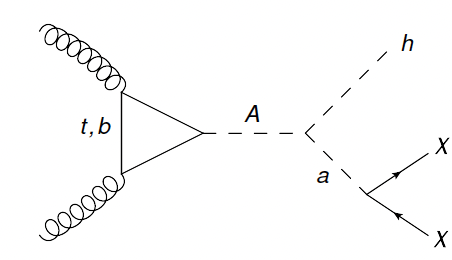
\includegraphics[width=0.7\linewidth]{2HDM_a}}
\end{minipage}
\begin{minipage}{0.32\linewidth}
\centerline{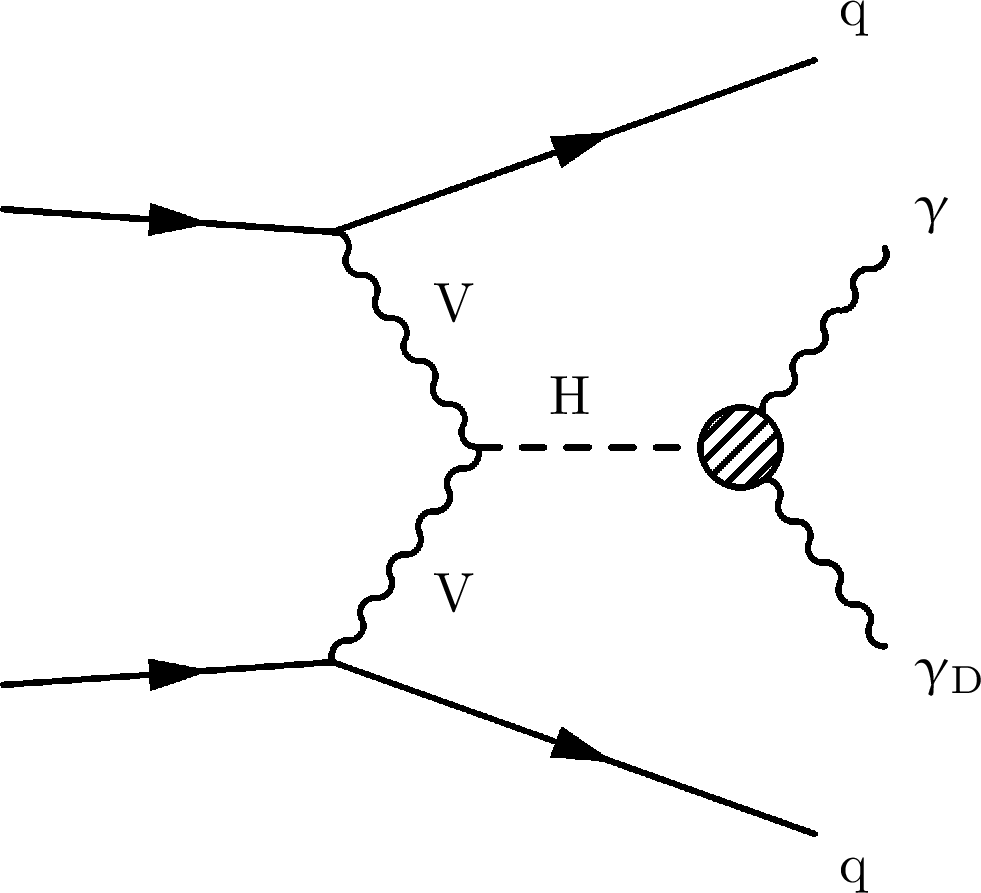
\includegraphics[width=0.7\linewidth]{HiggsDarkPhotonDiagram}}
\end{minipage}
\begin{minipage}{0.32\linewidth}
\centerline{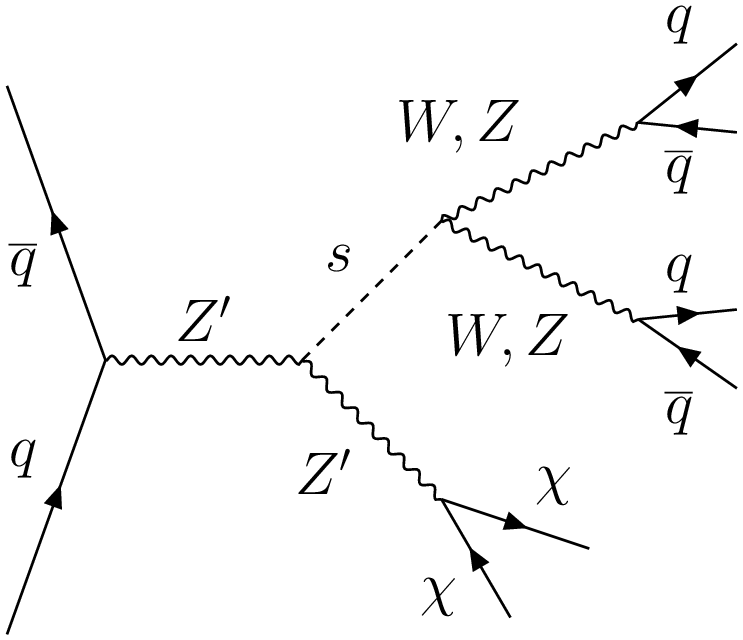
\includegraphics[width=0.7\linewidth]{MonoSVVDiagram}}
\end{minipage}
\caption[]{Diagrams of various models considered in recent DM searches. Left: A Higgs boson is produced in association with a pseudo-scalar (a) decaying to DM candidates (2HDM+a); middle: a Higgs boson is produced in the VHF channel, decaying to a photon and a dark photon; right: a dark Higgs s is produced in association with a $Z^{\prime}$, where the $Z^{\prime}$ decays to DM candidates and the dark Higgs decays to two vector bosons.}
\label{fig:diagrams}
\end{figure}

Recent results from both CMS and ATLAS will be summarized in the next section
followed by an outlook on the future DM search programs at the LHC. All
searches discussed in this article use full Run 2 dataset. 

\section{Dedicated search results}

\subsection{Mono-X searches}

The mono-jet search is the flagship analysis in the DM search program as its final
state covers a large range of the parameter space, sensitive to many different
models. The recent ATLAS mono-jet search~\cite{monojet} uses data collected by a missing transverse energy, $\et$,
trigger. The events are required to have at least one energetic jet and not
have leptons or photons present. Signal regions are divided by $\et$\ and various control regions are constructed by allowing leptons. A simultaneous fit is performed in both the signal regions and control regions, and the resulting discriminant spectrum expected from the background is compared with data to determine whether there are significant deviations in the latter. This simultaneous fit strategy is a common procedure adopted by all the searches discussed in this article.

The mono-$Z$ search is also a very important inclusive analysis. The recent CMS mono-$Z$
search~\cite{monoz} considers the leptonic final state where the $Z$ boson
decays to either a pair of muons or electrons. Events are collected by di-muon
(di-electron) triggers and must contain two well-identified, isolated muons
(electrons) with the same flavor and opposite charge, forming an invariant mass
compatible with the $Z$ boson mass. Events with additional leptons, more than
one jet or any $b$-tagged jets are vetoed to suppress the backgrounds. Signal
regions are constructed based on either the missing transverse momentum,
$\ptmiss$, or the transverse mass between the di-lepton system and $\ptmiss$,
$\mt$. The latter region is optimized for 2HDM+a model as there is a peak in $\mt$
spectrum near the neutral scalar (H) mass.

Both the mono-jet and mono-$Z$ searches have data observation compatible with the background estimations and upper limits are set on specific models as the examples shown in Figure~\ref{fig:mono_jet_z}. 

\begin{figure} [htb]
\begin{minipage}{0.45\linewidth}
\centerline{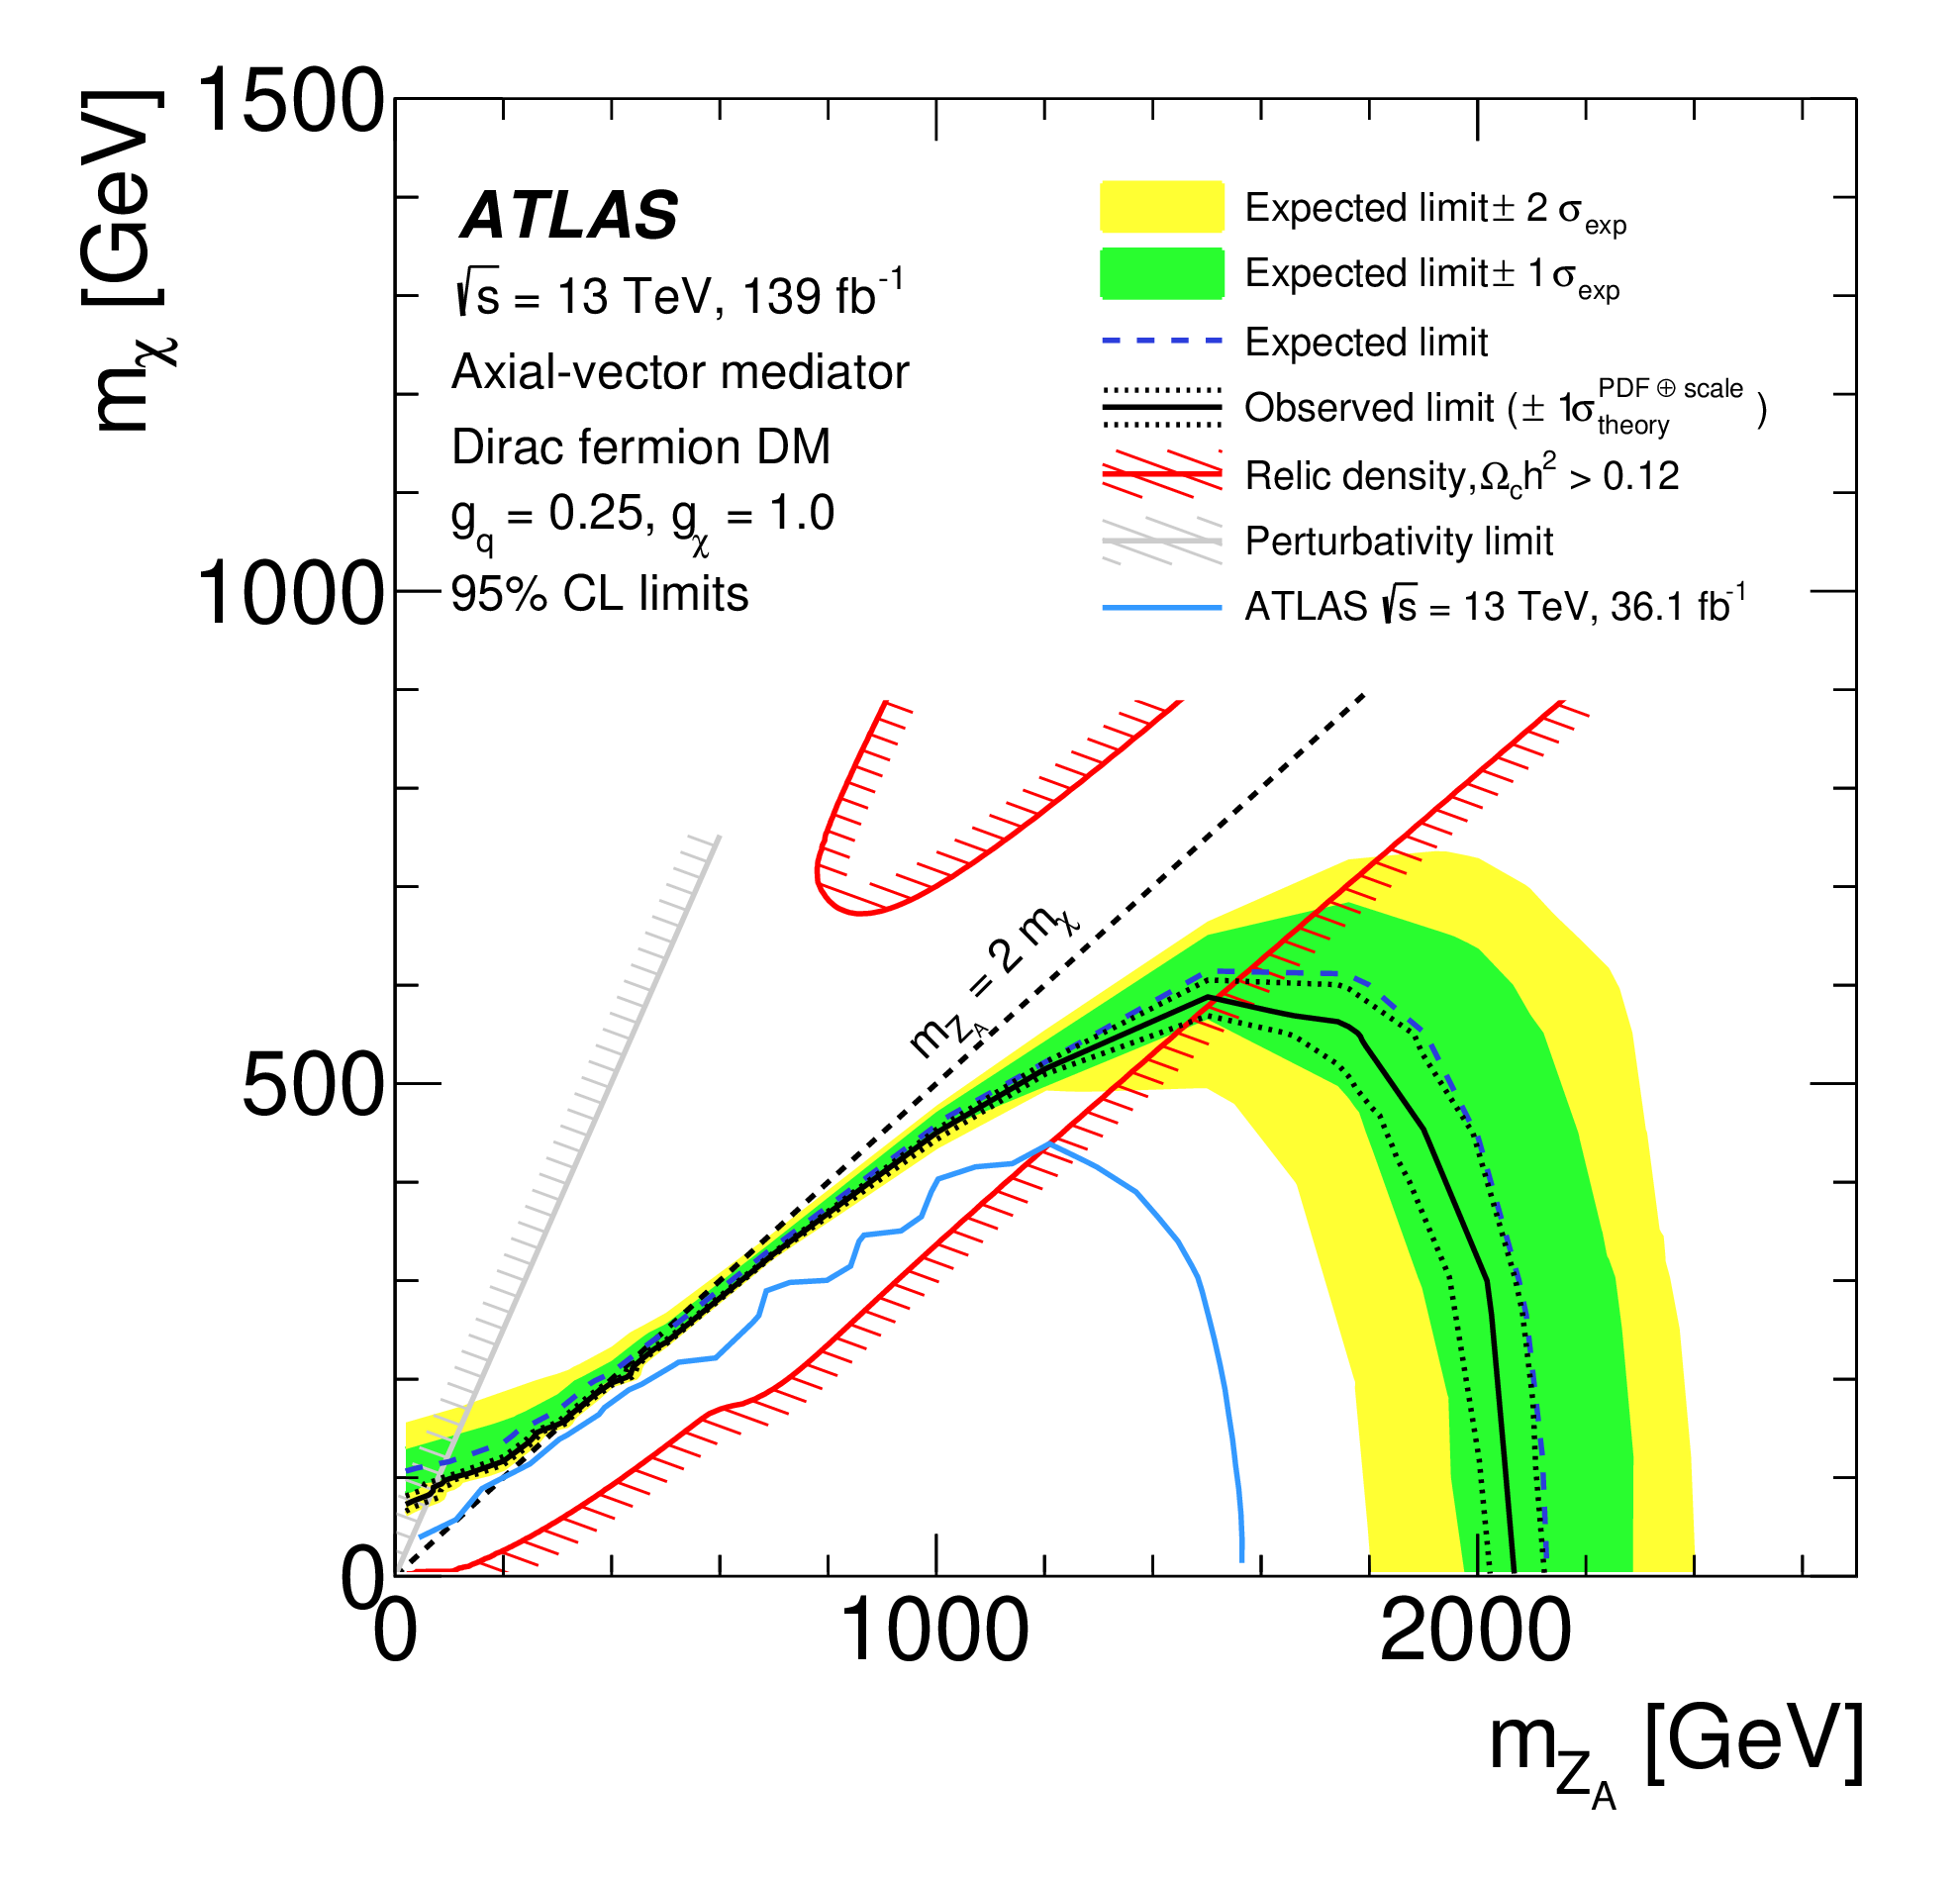
\includegraphics[width=0.8\linewidth]{monojet}}
\end{minipage}
\begin{minipage}{0.45\linewidth}
\centerline{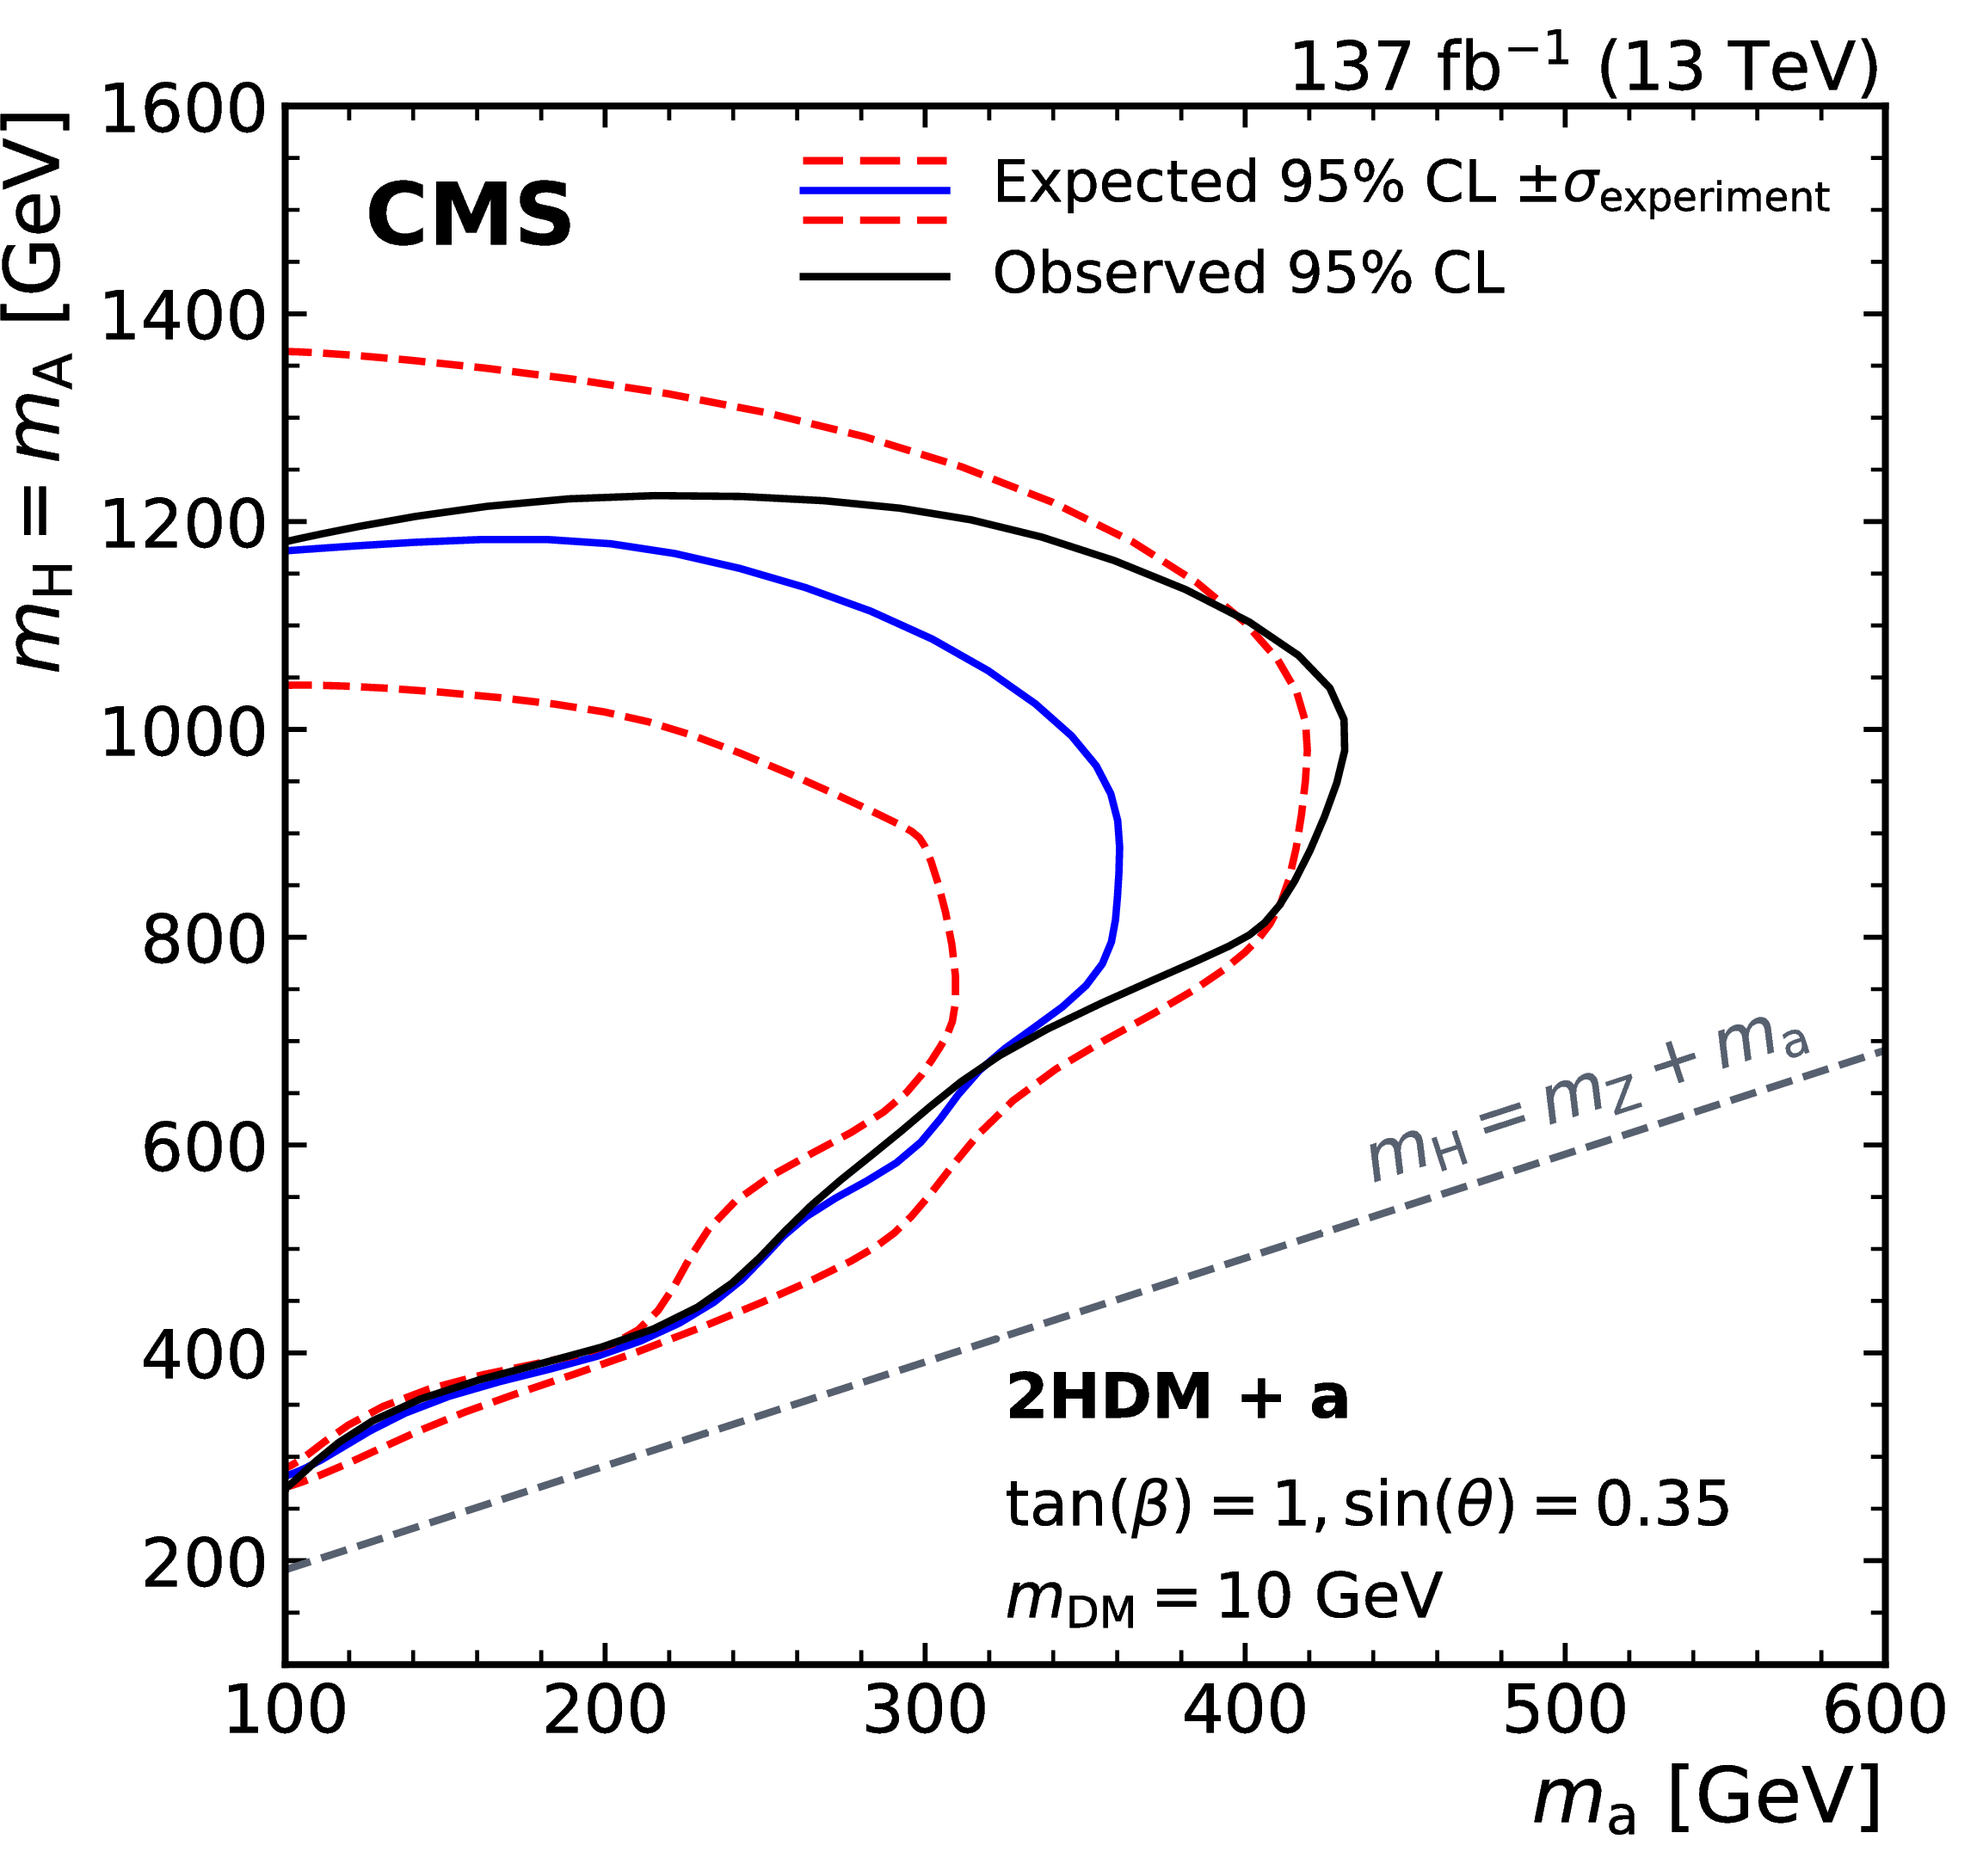
\includegraphics[width=0.8\linewidth]{monoz}}
\end{minipage}
\caption[]{Left: observed (solid) and expected (dashed) limits on the axial-vector mediator masses obtained in the mono-jet search~\cite{monojet}. The $y$-axis corresponds to the dark matter mass ($m_{\chi}$) while the $x$-axis refers to the axial-vector mass ($m_{Z_{\mathrm{A}}}$). Right: observed (solid) and expected (dashed) limits on the 2HDM+a model obtained in the mono-$Z$ search~\cite{monoz}. The $y$-axis corresponds to the neutral scalar mass ($m_{\mathrm{H}}$) while the $x$-axis refers to the pseudo-scalar mass ($m_{\mathrm{a}}$).}
\label{fig:mono_jet_z}
\end{figure}

Both the mono-jet and mono-$Z$ search consider well known detectable standard
model (SM) physic objects. Searches considering less well known SM particles
such as the Higgs boson or new BSM particles such as new scalar particles target particular phase space, facing different experimental challenges. The recent
ATLAS mono-Higgs($\rightarrow b\overline{b}$) search~\cite{monoh} analyzes
events collected by the primary $\et$\ triggers. Events are required to have
a significant $\et$\ above the trigger threshold and not contain isolated leptons. The signal regions are categorized by
the $b$-tagged jet multiplicity (two or three) and the collinearity of the two
$b$-tagged jets forming the Higgs candidate (merged and resolved). The ATLAS
mono-s($\rightarrow VV$) search~\cite{monos} probes a similar final state but looks for hadronic boson decays instead of $b$-hadron
decays. Events must contain two boson-tagged jets, and the signal regions are
categorized by their collinearity (merged and intermediate) as well. 

Data observation agrees well with the background expectation in both the mono-Higgs($\rightarrow b\overline{b}$) and mono-s($\rightarrow VV$) searches. Upper limits are set on specific models as the examples shown in Figure~\ref{fig:mono_h_s}.      

\begin{figure} [htb]
\begin{minipage}{0.45\linewidth}
\centerline{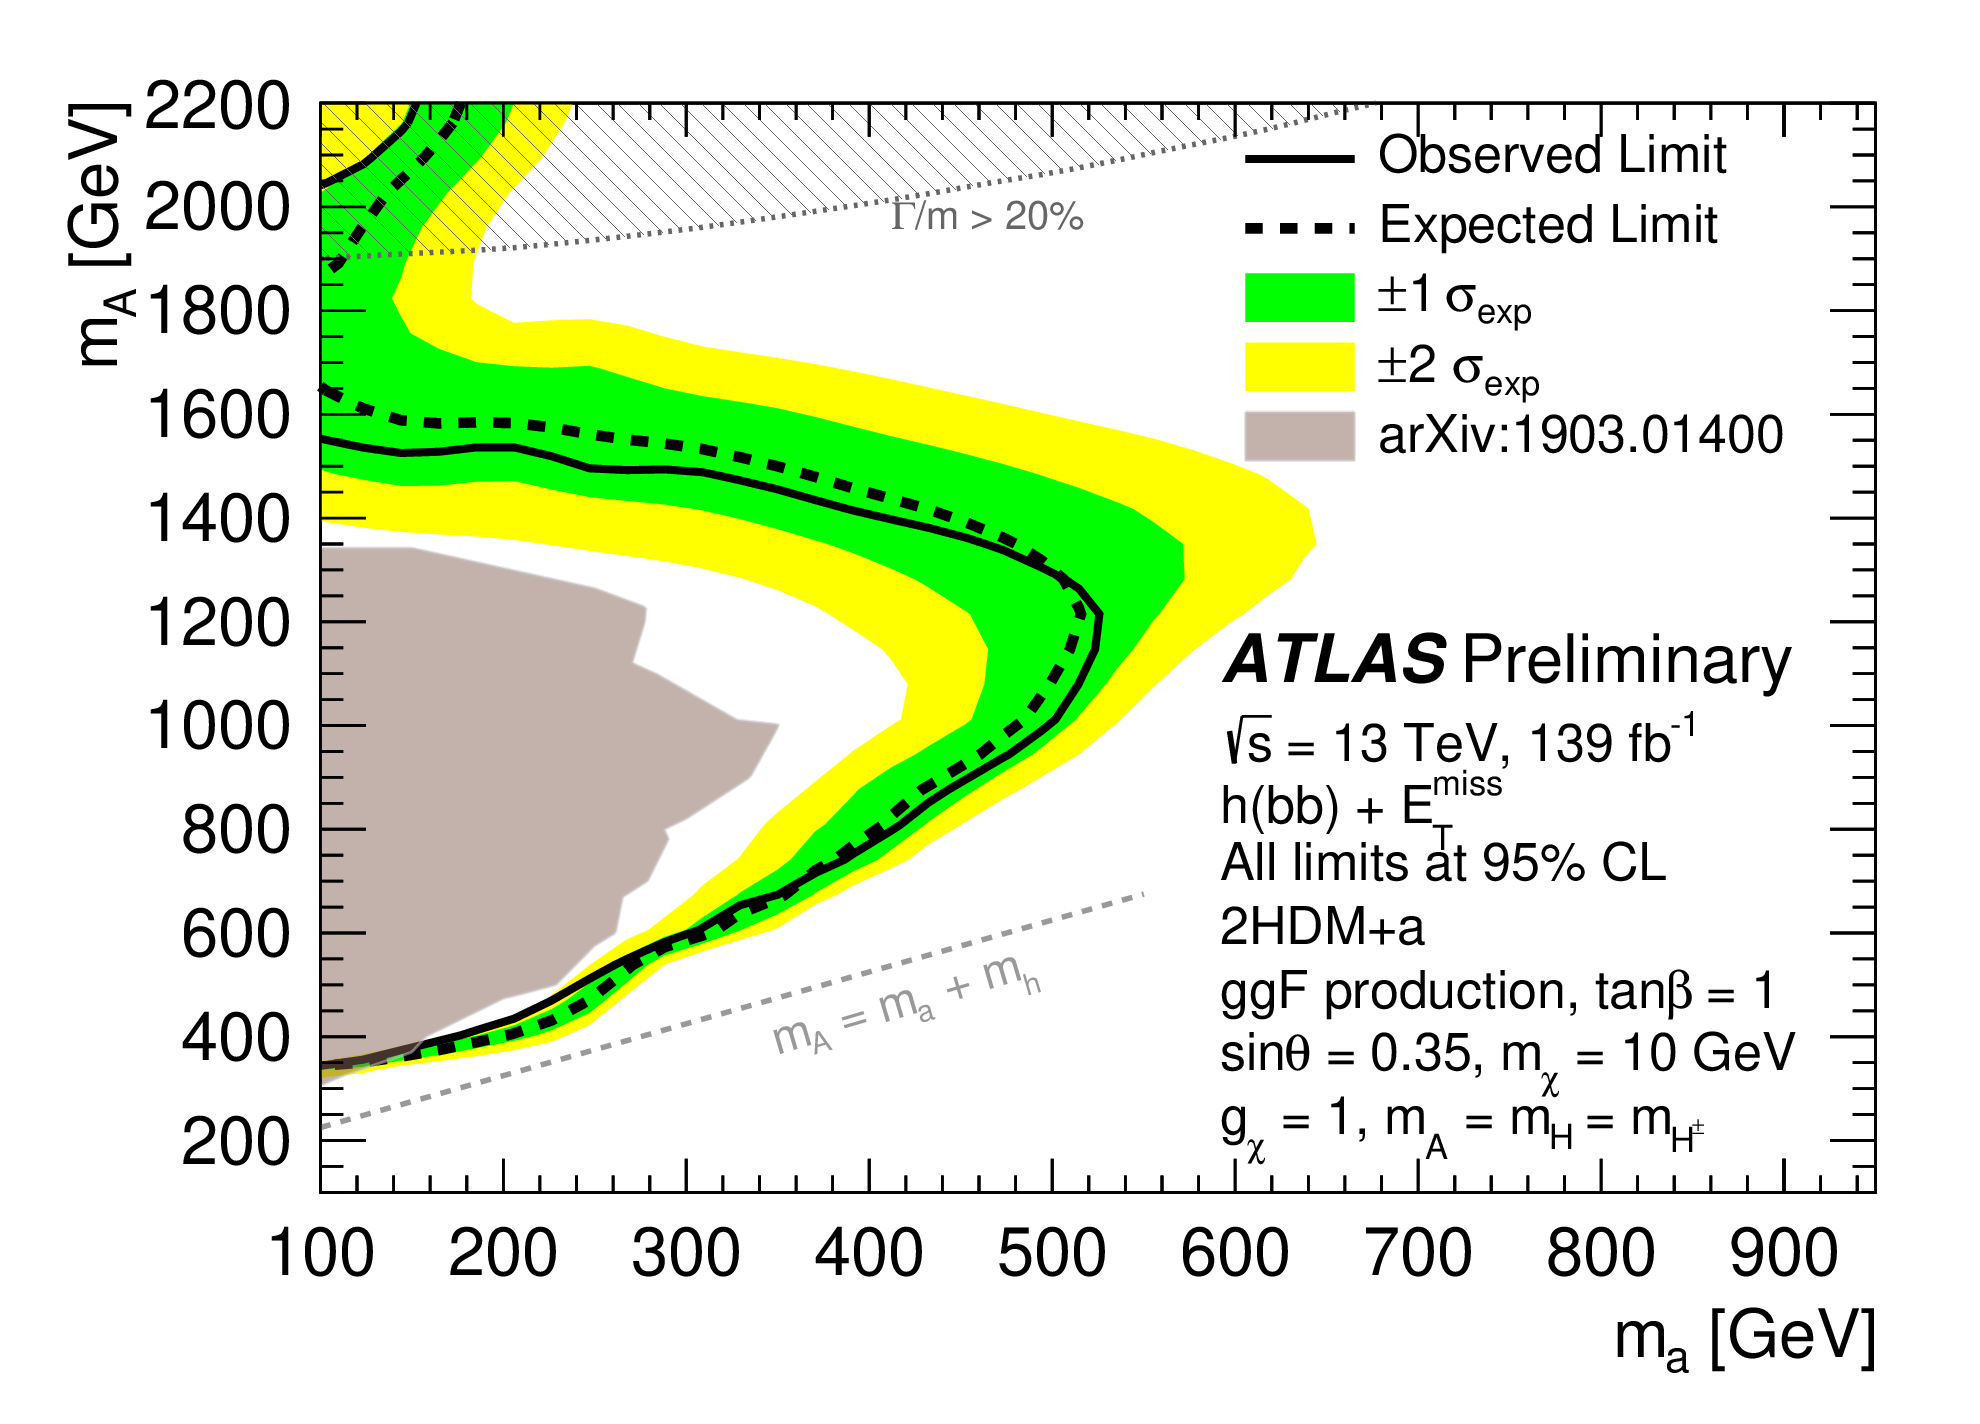
\includegraphics[width=0.8\linewidth]{monoh}}
\end{minipage}
\begin{minipage}{0.45\linewidth}
\centerline{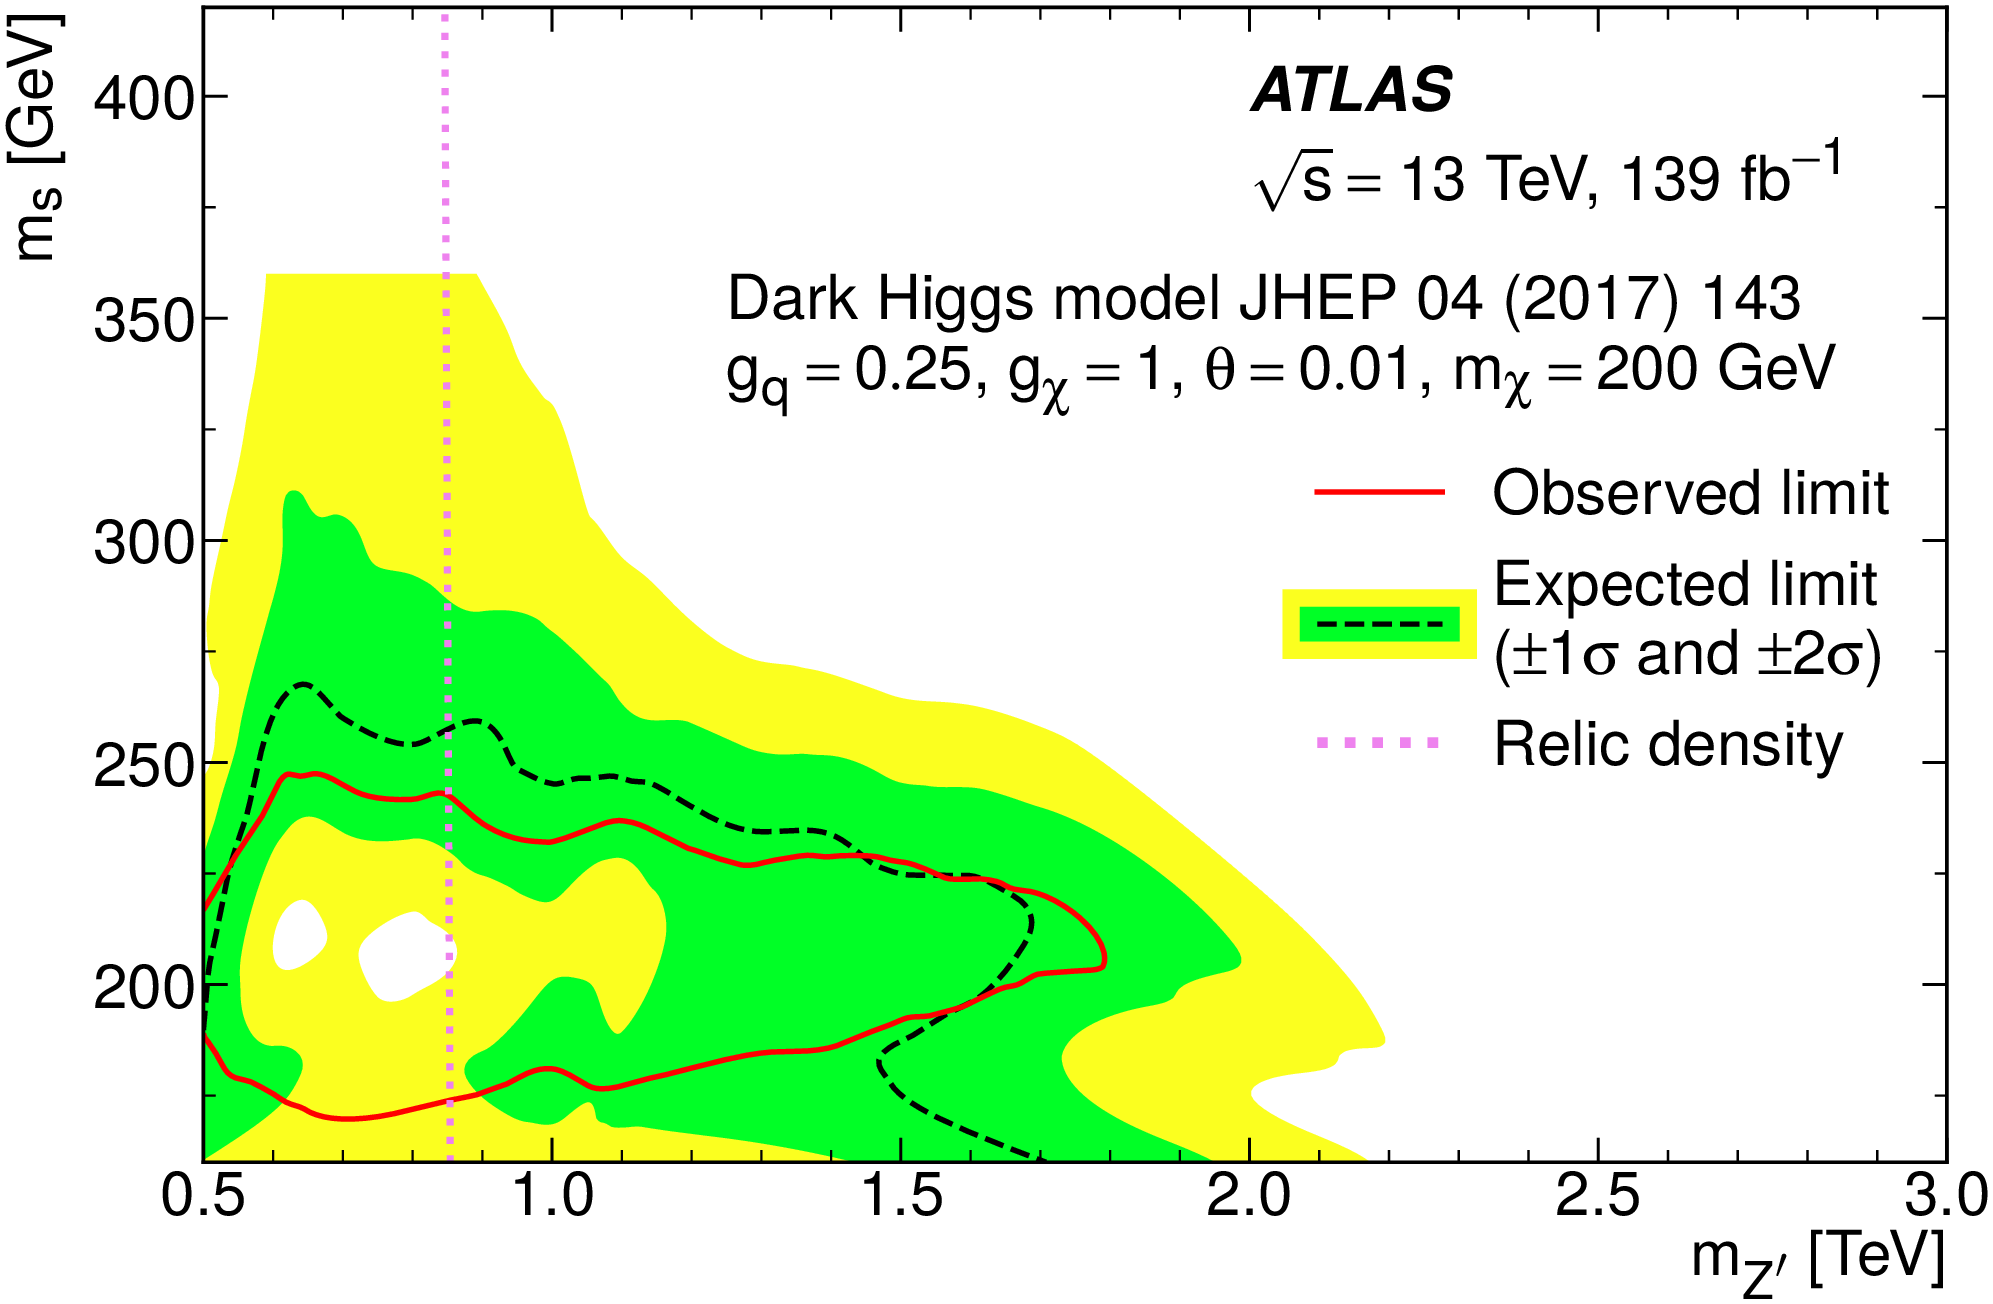
\includegraphics[width=0.8\linewidth]{monos}}
\end{minipage}
\caption[]{Left: observed (solid) and expected (dashed) limits on the 2HDM+a model obtained in the mono-H($\rightarrow b\overline{b}$) search~\cite{monoh}. The $y$-axis corresponds to the heavy Higgs boson mass ($m_{\mathrm{A}}$) and the $x$-axis refers to the pseudo-scalar mass $m_{\mathrm{a}}$. Right: observed (solid) and expected (dashed) limits on the dark Higgs model obtained in the mono-s($\rightarrow VV$) search~\cite{monos}. The $y$-axis corresponds to the dark Higgs boson mass ($m_{\mathrm{s}}$) and the $x$-axis refers to the $Z^{\prime}$ mass $m_{Z^{\prime}}$.}
\label{fig:mono_h_s}
\end{figure}

\subsection{Dark photon search in the vector boson fusion (VBF) channel}

As the most recently discovered SM particle, the Higgs boson opens up an
interesting avenue for DM search, not only because it can be produced in
association with DM particles but also it may decay to DM particles. The
invisible Higgs decay branching ratio is a critical channel to study the
phase space where $m_{\mathrm{DM}} < \frac{1}{2}m_{\mathrm{H}}$. The invisible Higgs decay branching ratio measurement~\cite{hinv} sets a stringent
upper limit of 0.11 at 95\% CL. Recent ATLAS~\cite{atlasvbf} and
CMS~\cite{cmsvbf} searches explore another unique scenario where the Higgs boson
decays to a dark photon and a photon, which gives a significant $\et$\ and a photon
in the final state. Both searches consider the VBF production channel given its
larger cross section, applying similar event selections such as containing VBF
jets and lepton veto. The $\mt$\ between the photon and the $\ptmiss$\ is used
as the discriminant variable to define the signal regions. 

No significant deviations are observed in both searches and upper limits are set on $\sigma_{\mathrm{VBF}}\times B(H\rightarrow\gamma+inv)$ as shown in Figure~\ref{fig:vbf}. It is worth mentioning that ATLAS applies a lower photon $p_{\mathrm{T}}$ threshold and
additional jet centrality requirements, resulting in stronger exclusion limits.  

\begin{figure} [htb]
\begin{minipage}{0.45\linewidth}
\centerline{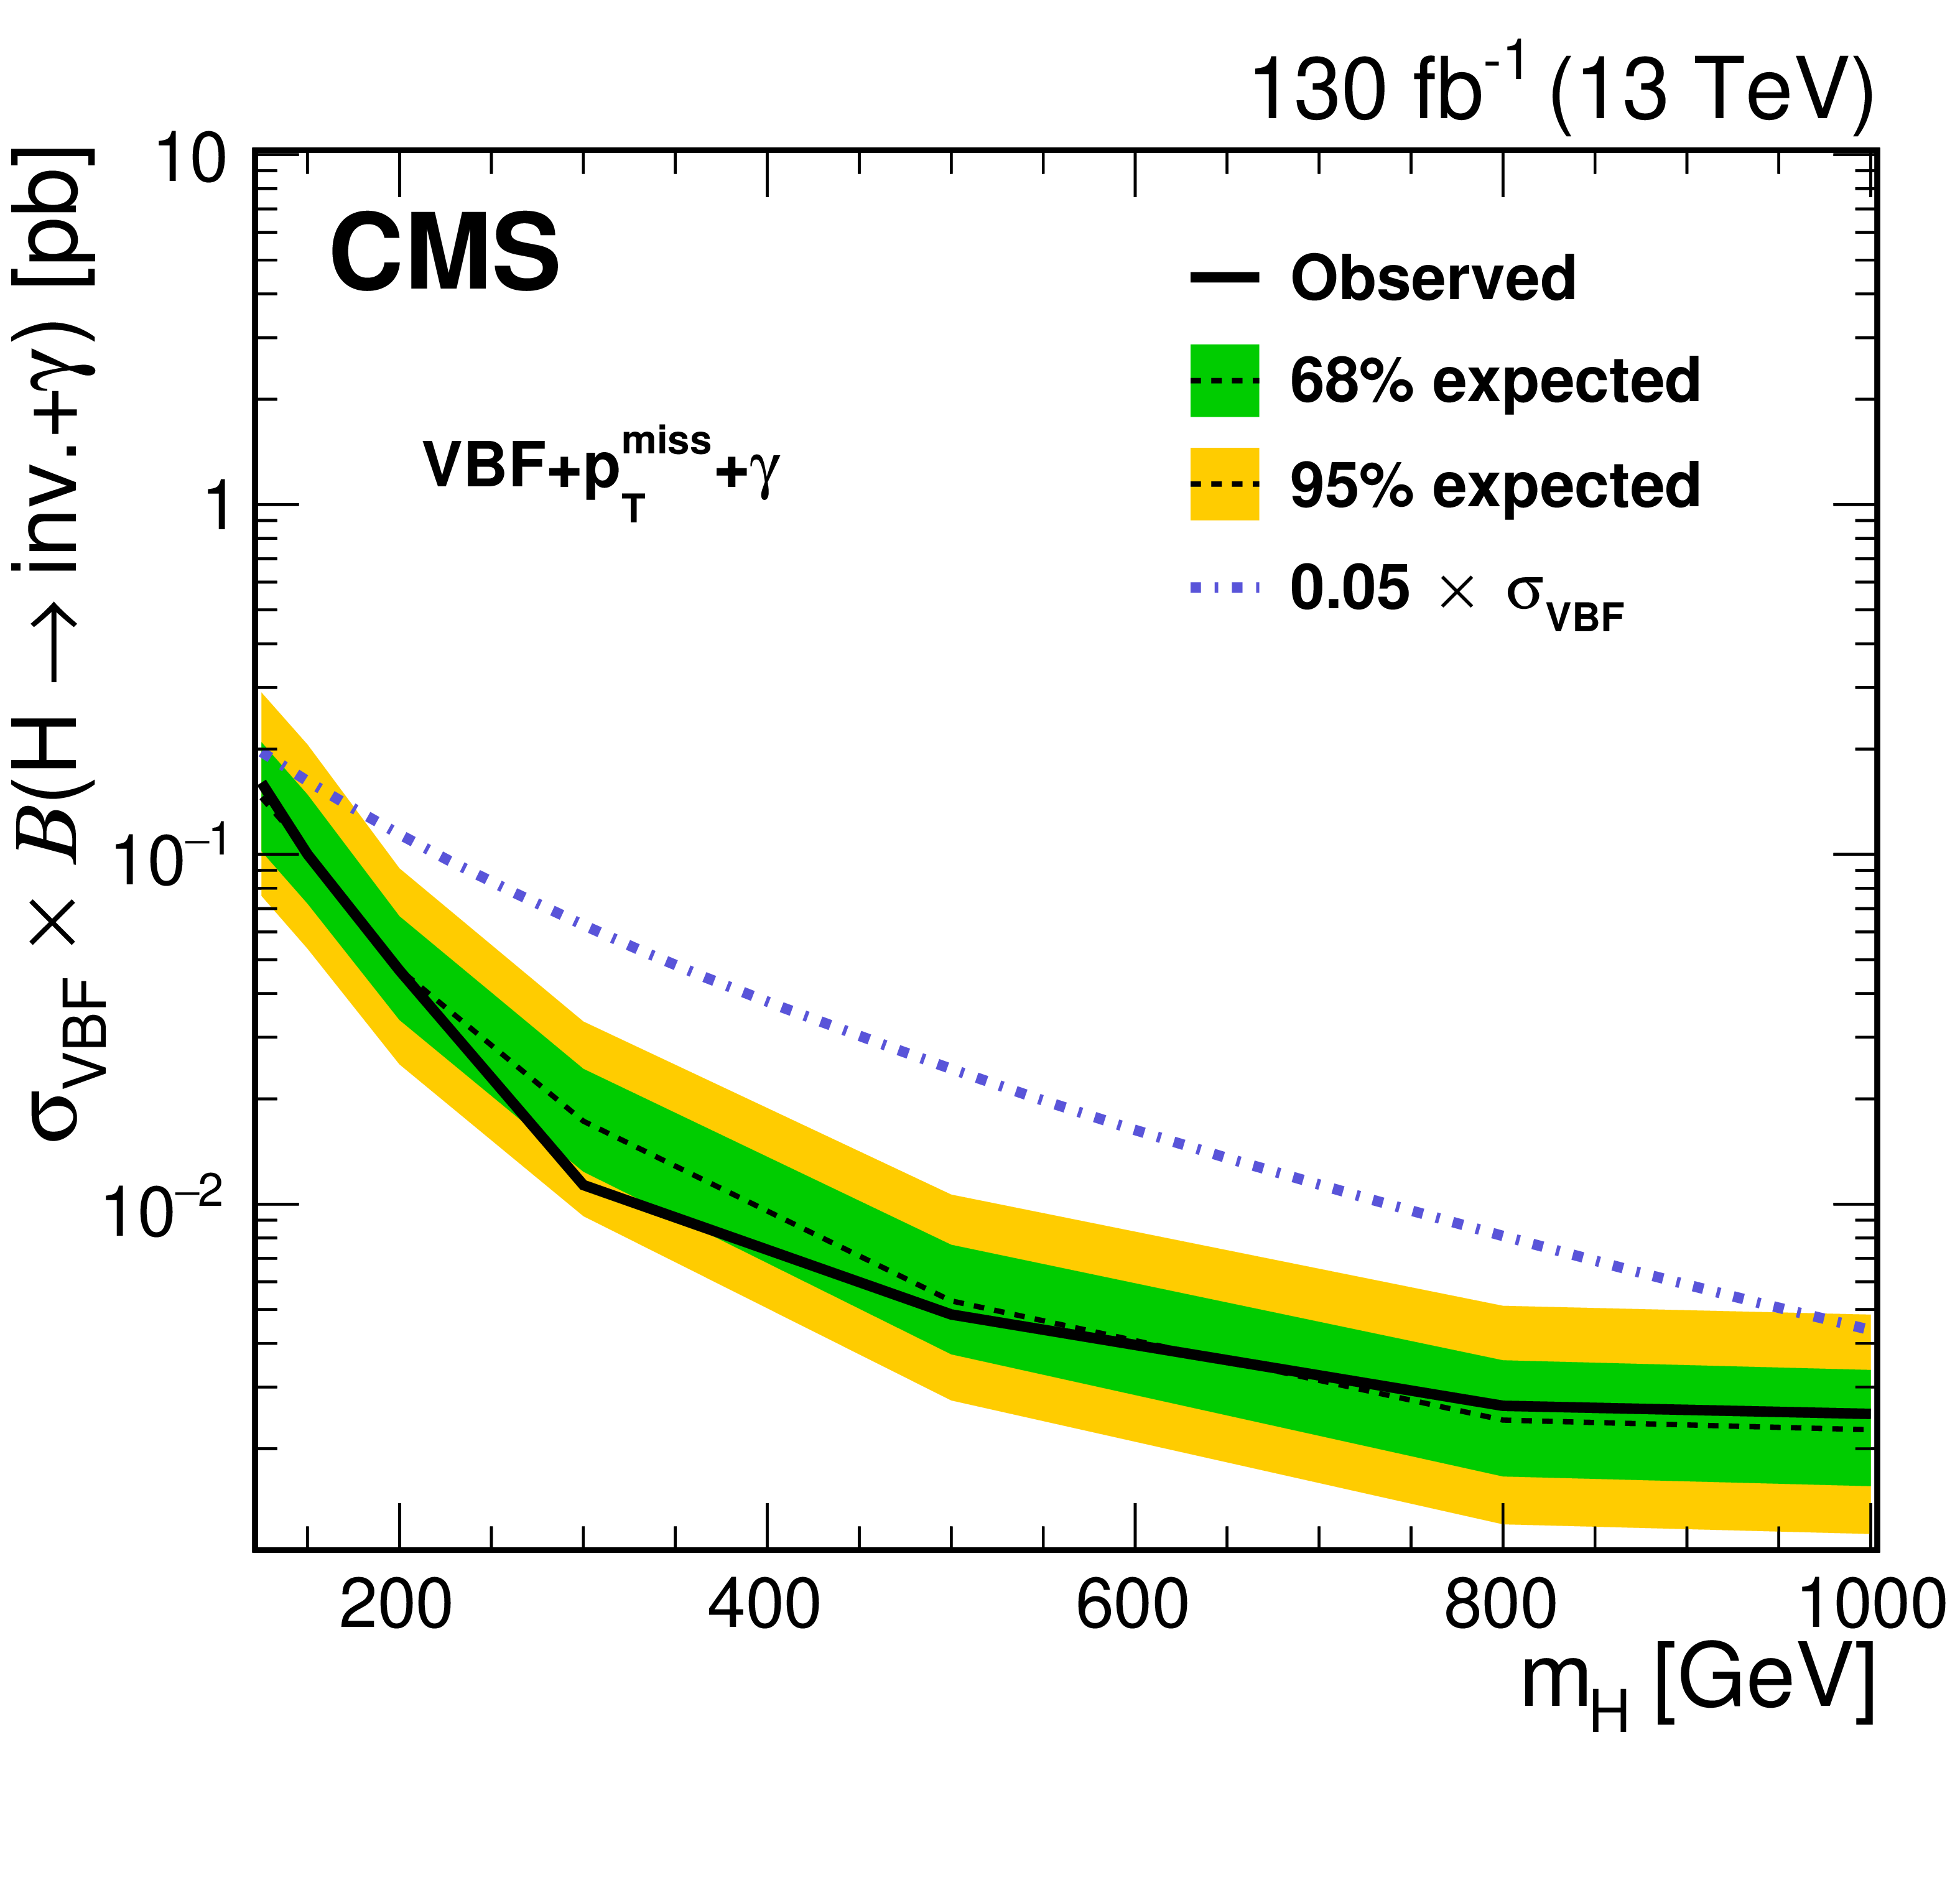
\includegraphics[width=0.8\linewidth]{cmsvbf}}
\end{minipage}
\begin{minipage}{0.5\linewidth}
\centerline{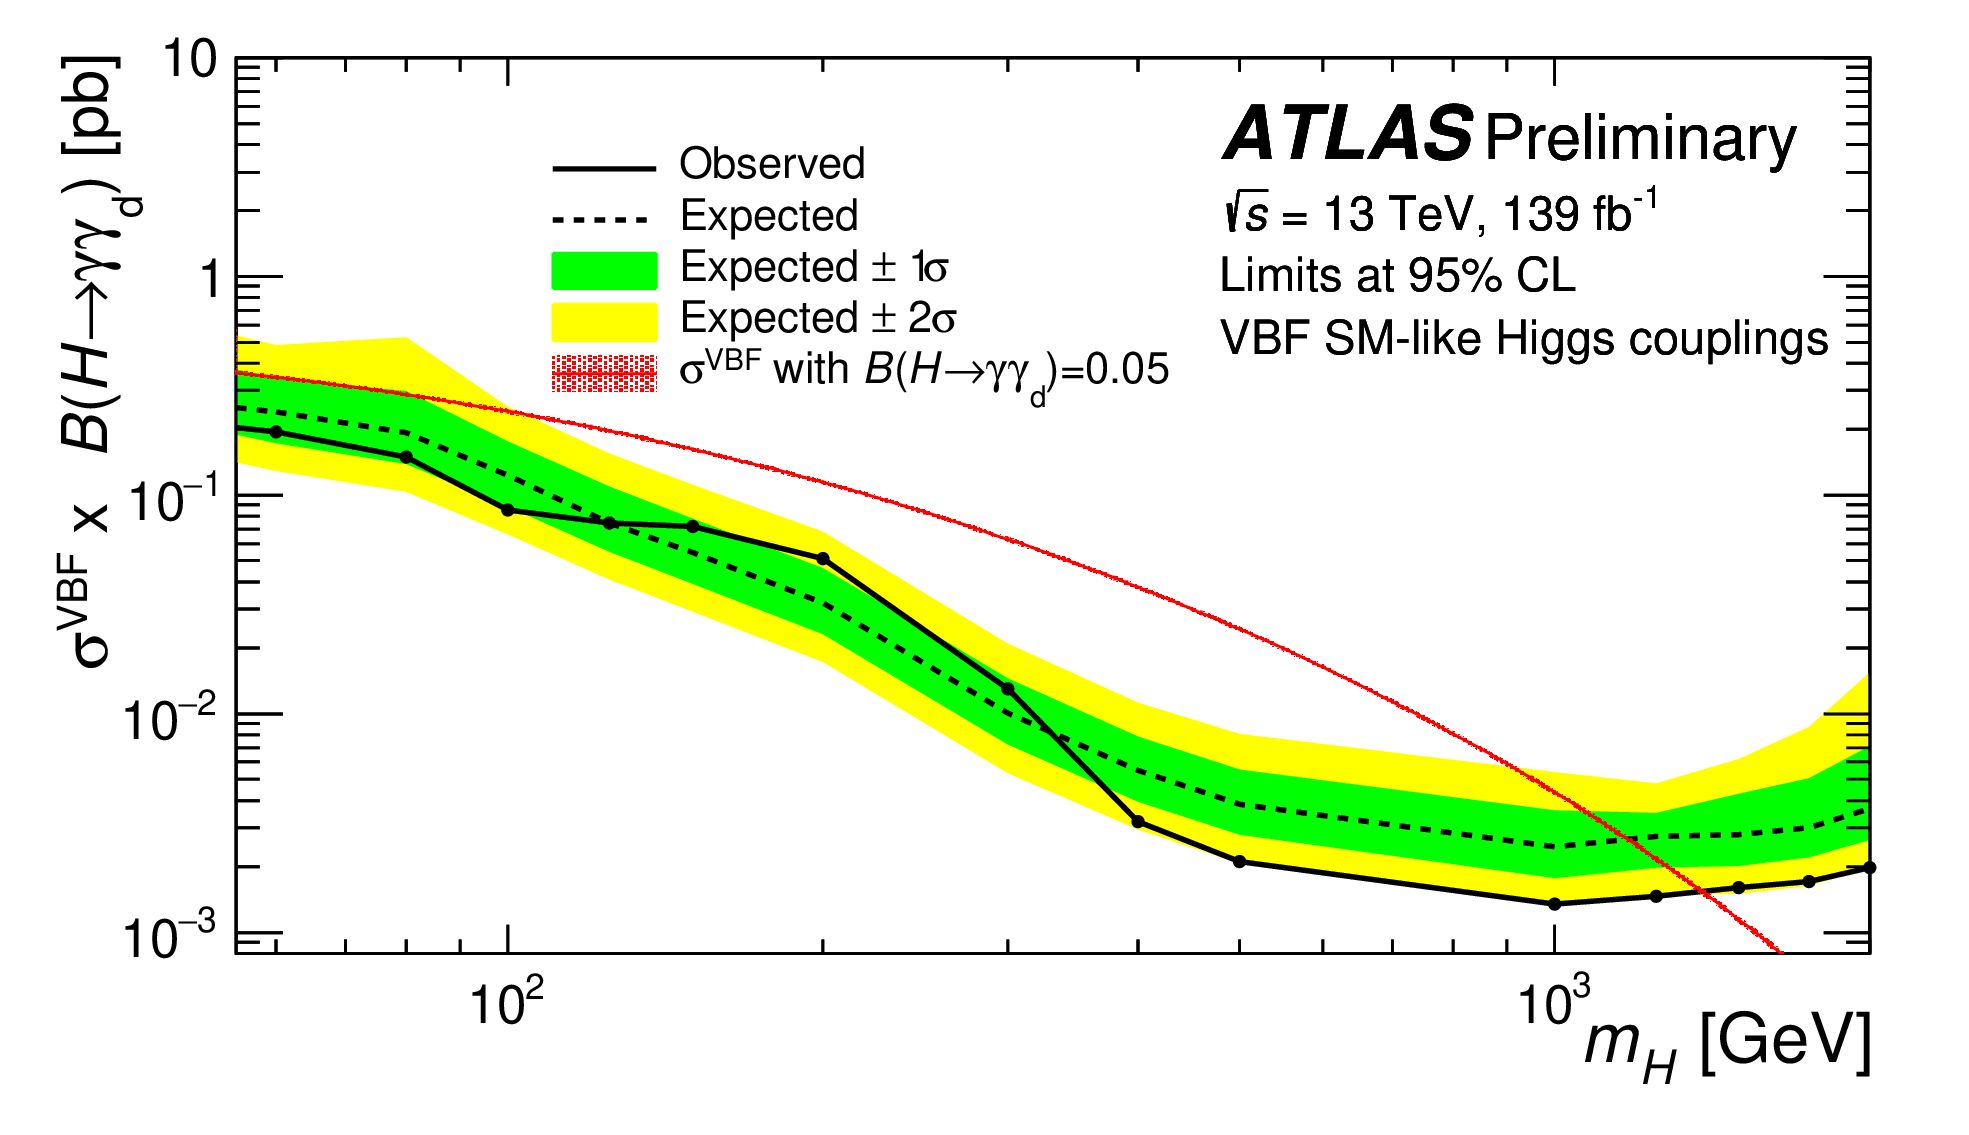
\includegraphics[width=1.0\linewidth]{atlasvbf}}
\end{minipage}
\caption[]{Observed (solid) and expected (dashed) limits on $\sigma_{\mathrm{VBF}}\times B(H\rightarrow\gamma+inv)$ obtained in the CMS~\cite{cmsvbf} (left) and ATLAS~\cite{atlasvbf} (right) search. The $x$-axis refers to the Higgs boson mass ($m_{\mathrm{H}}$).}
\label{fig:vbf}
\end{figure}

\subsection{DM interpretations in SUSY searches}

R-parity conserving (RPC) SUSY predicts a stable lightest supersymmetric
particle (LSP), which is a good DM candidate. SUSY searches targeting this
scenario usually requires large $\et$ and high jet ($b$-tagged jet)
multiplicity. Certain DM models share similar final states. In a recent ATLAS
SUSY search~\cite{dmbb}, dedicated signal regions are constructed and optimized
for DM particles produced in association with a pair of $b$-quarks. Event
selections include $\et$, $b$-jet multiplicity and lepton veto. In addition,
specialized variables exploring the angular correlations are applied to optimize individual signal regions. The
background prediction agrees well with the data, therefore upper limits are set
on the DM production cross section as shown in Figure~\ref{fig:dmbb}.   

\begin{figure} [htb]
\centerline{\includegraphics[width=0.5\linewidth]{DMBB}}
\caption[]{Observed (solid) and expected (dashed) limits on the DM cross section obtained in the ATLAS SUSY search~\cite{dmbb}. The $x$-axis refers to the mediator mass ($m_{\mathrm{a}}$) and the $y$-axis is the cross-section divided by the theoretical prediction.}
\label{fig:dmbb}
\end{figure}

\section{Conclusions}

The LHC experiments have explored a very large phase space where DM could have existed.  Recent
theoretical development encourages searches to look at more specific final
states in addition to the inclusive ones and several new results from both CMS
and ATLAS already extended the scope of the DM search program to new horizons.
There are still many ongoing full Run 2 DM searches that will further broaden
the coverage. More dedicated triggers and reconstruction technologies are
being developed to improve the search sensitivities. 

\section*{References}

\begin{thebibliography}{99}

\bibitem{LHCRef}L. Evans and P. Bryant (editors), \Journal{\JINST}{3}{S08001}{2008}.

\bibitem{CMSRef}CMS Collaboration, \Journal{\JINST}{3}{S08004}{2008}.

\bibitem{ATLASRef}ATLAS Collaboration, \Journal{\JINST}{3}{S08003}{2008}.

\bibitem{DarkH}Duerr, Michael and Grohsjean, Alexander and Kahlhoefer, Felix and Penning, Bjoern and Schmidt-Hoberg, Kai and Schwanenberger, Christian, \Journal{\JHEP}{04}{143}{2017}.

\bibitem{DarkPh}Biswas, Sanjoy and Gabrielli, Emidio and Heikinheimo, Matti and Mele, Barbara, \Journal{\PRD}{93}{093011}{2016}.

\bibitem{2HDM}Bauer, M., Haisch, U. and Kahlhoefer, F., \Journal{\JHEP}{05}{138}{2017}.

\bibitem{monojet}ATLAS Collaboration, CERN-EP-2020-238, https://cds.cern.ch/record/2752675.

\bibitem{monoz}CMS Collaboration, \Journal{\EPJC}{81}{13}{2021}.

\bibitem{monoh}ATLAS Collaboration, ATLAS-CONF-2021-006, http://cdsweb.cern.ch/record/2759211. 

\bibitem{monos}ATLAS Collaboration, \Journal{\PRL}{126}{121802}{2021} 

\bibitem{hinv}ATLAS Collaboration, ATLAS-CONF-2020-052, https://cds.cern.ch/record/2743055.

\bibitem{cmsvbf}CMS Collaboration, \Journal{\JHEP}{03}{011}{2021}.

\bibitem{atlasvbf}ATLAS Collaboration, ATLAS-CONF-2021-004, http://cdsweb.cern.ch/record/2758212.

\bibitem{dmbb}ATLAS Collaboration, CERN-EP-2021-001, https://cds.cern.ch/record/2750578.

\end{thebibliography}

\end{document}

%%%%%%%%%%%%%%%%%%%%%%
% End of moriond.tex  %
%%%%%%%%%%%%%%%%%%%%%%


%%% Local Variables: 
%%% mode: latex
%%% TeX-master: t
%%% End: 

%%% Local Variables: 
%%% mode: latex
%%% TeX-master: t
%%% End: 

%%% Local Variables: 
%%% mode: latex
%%% TeX-master: t
%%% End: 
